\chapter{AnemoI – AI-Based Weather Modeling}

%==============================================================================
%
%==============================================================================
\section{Yaml, Hydra and OmegaConf}

Before we explore AnemoI let us complete our preparation by looking at two main tools used. 

%------------------------------------------------------------------------------
%
%------------------------------------------------------------------------------
\subsection{YAML – Configuration Made Simple}

YAML (YAML Ain't Markup Language) is a human-readable format used for configuration files. It is built on indentation and simple key-value structures, making it ideal for defining settings in machine learning workflows.

In the context of Anemoi and many other ML frameworks, YAML is used to define model parameters, training hyperparameters, and paths. Here's a simple YAML file that defines both a model and a training configuration:

\begin{codeonly}{Model and Training Configuration}
model:
  name: simple_model
  input_size: 10
  hidden_size: 20
  output_size: 1

training:
  epochs: 5
  batch_size: 32
  learning_rate: 0.01
\end{codeonly}

This configuration can be loaded in Python using the \texttt{PyYAML} library and interpreted as a dictionary. Here's an example of how to load it:

\begin{codeonly}{Python: Load YAML}
import yaml

with open("simple_config.yaml", "r") as file:
    config = yaml.safe_load(file)

print("Model name:", config["model"]["name"])
print("Training for", config["training"]["epochs"], "epochs")
\end{codeonly}

You can then pass this configuration into a training function or class:

\begin{codeonly}{Python: Use Configuration}
def train_model(config):
    print(f"Training model '{config['model']['name']}'")
    print("Hyperparameters:")
    print("  Learning rate:", config["training"]["learning_rate"])
    print("  Batch size:", config["training"]["batch_size"])
    for epoch in range(config["training"]["epochs"]):
        print(f"Epoch {epoch+1}... (training logic here)")

train_model(config)
\end{codeonly}

This illustrates how YAML is used as an external, editable source of parameters for training code, enabling experiment reproducibility and flexible configuration.

%------------------------------------------------------------------------------
%
%------------------------------------------------------------------------------
\subsection{Hydra – Flexible Configuration for ML Experiments}

Hydra is a Python framework for managing complex configuration workflows. It allows users to compose and override YAML configuration files at runtime, enabling modular and reusable setups for machine learning experiments. In our example, we train a neural network to learn the function \( y = \sin(x) \), and use Hydra to flexibly switch between different model architectures and training parameters.

\begin{figure}[ht]
  \centering
  \begin{minipage}{0.48\textwidth}
    \centering
    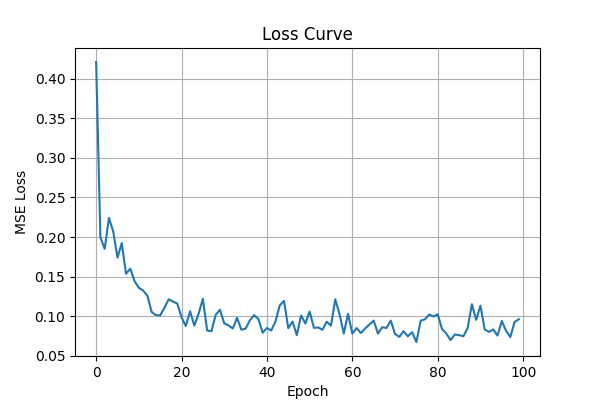
\includegraphics[width=\linewidth]{images/hydra1_mlp.png}
    \caption*{{\bf (a)} Loss curve for the shallow model (\texttt{mlp}). Training converges quickly to a low loss.}
  \end{minipage}
  \hfill
  \begin{minipage}{0.48\textwidth}
    \centering
    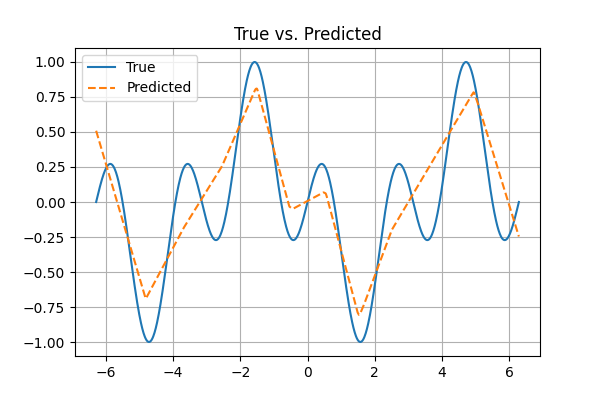
\includegraphics[width=\linewidth]{images/hydra2_mlp.png}
    \caption*{{\bf (b)} Prediction result for the shallow model. The curve closely matches the true $\sin(x)$ target.}
  \end{minipage}

  \vspace{1em}

  \begin{minipage}{0.48\textwidth}
    \centering
    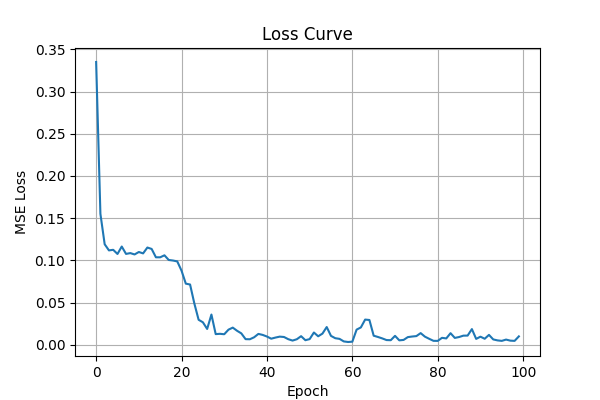
\includegraphics[width=\linewidth]{images/hydra1_deep.png}
    \caption*{{\bf (c)} Loss curve for the deeper model (\texttt{deep}). Training is slower and convergence less stable.}
  \end{minipage}
  \hfill
  \begin{minipage}{0.48\textwidth}
    \centering
    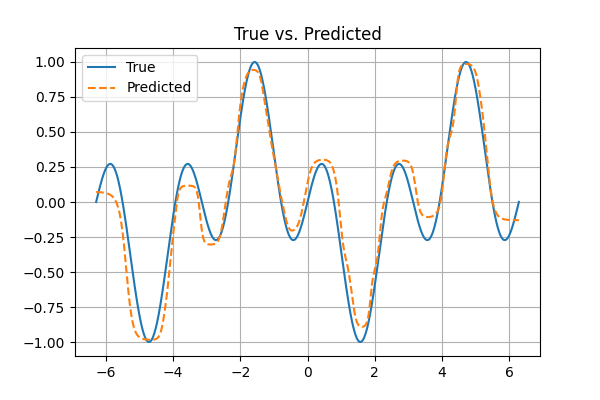
\includegraphics[width=\linewidth]{images/hydra2_deep.png}
    \caption*{{\bf (d)} Prediction result for the deeper model. The curve is less smooth and overshoots the target in places.}
  \end{minipage}

  \caption{Training results for two model configurations defined using Hydra. The shallow model (\texttt{mlp}) performs more effectively for approximating the simple $\sin(x)$ function, while the deeper model (\texttt{deep}) shows signs of overfitting or instability.}
  \label{fig:hydra-mlp-comparison}
\end{figure}


{\bf Base Configuration:} The central Hydra entry point is \texttt{config.yaml}, which specifies which model and training configuration to load:

\begin{codeonly}{config.yaml}
defaults:
  - model: mlp
  - training: simple
  - _self_
\end{codeonly}

{\bf Shallow MLP Configuration:} A simple neural network with one hidden layer is defined like this:

\begin{codeonly}{model/mlp.yaml}
layer_sizes: [1, 64, 1]
activation: relu
\end{codeonly}

{\bf Deeper Network Configuration:} A deeper network with three hidden layers can be defined similarly:

\begin{codeonly}{model/deep.yaml}
layer_sizes: [1, 128, 64, 32, 1]
activation: tanh
\end{codeonly}

{\bf Training Configuration:} Training hyperparameters such as learning rate and batch size are defined in a separate file:

\begin{codeonly}{training/simple.yaml}
epochs: 100
lr: 0.01
batch_size: 32
\end{codeonly}

{\bf Using Hydra in Python:} Hydra supports programmatic configuration loading and overrides using the \texttt{initialize} and \texttt{compose} functions. This allows the configuration to be composed dynamically at runtime, for example to switch between different models within the same training loop.

In the following example, the \texttt{run\_with\_override} function dynamically loads a specified model configuration (e.g., \texttt{mlp} or \texttt{deep}) and then trains the model accordingly.

\begin{codeonly}{Python}
from hydra import initialize, compose

def run_with_override(model_name, title):
    with initialize(config_path="conf", version_base=None):
        cfg = compose(config_name="config", overrides=[f"model={model_name}"])
    print(f"\\n{'='*30}\\nTraining model: {model_name.upper()} ({title})\\n{'='*30}")
    train_model(cfg)

# Run shallow model
run_with_override("mlp", "Shallow Network (1 hidden layer)")
\end{codeonly}

This function uses the Hydra override mechanism:
\begin{codeonly}{Python}
cfg = compose(config_name="config", overrides=[f"model={model_name}"])
\end{codeonly}
to replace the model defined in \texttt{config.yaml} at runtime. For example, if \texttt{model=deep} is used as an override, then \texttt{conf/model/deep.yaml} is loaded instead of the default \texttt{mlp.yaml}.

To demonstrate this in practice, the following snippet dynamically creates a deeper model configuration file (if not already present) and then runs training with it:

\begin{codeonly}{Python}
# Create deep model config if not already created
import os
if not os.path.exists("conf/model/deep.yaml"):
    with open("conf/model/deep.yaml", "w") as f:
        f.write(\"\"\"
layer_sizes: [1, 128, 64, 32, 1]
activation: tanh
\"\"\")

# Run deeper model
run_with_override("deep", "Deeper Network (3 hidden layers)")
\end{codeonly}

This dynamic Hydra setup makes it easy to test and compare different model architectures or training configurations without modifying the underlying training code. It supports flexible experimentation and reproducibility, which is particularly important in complex machine learning pipelines like Anemoi.

%------------------------------------------------------------------------------
%
%------------------------------------------------------------------------------
\subsection{OmegaConf Integration}

Internally, Anemoi relies on \texttt{OmegaConf} to represent and manipulate the hierarchical configuration tree provided by Hydra. Configuration classes like \texttt{BaseSchema} are converted to and from \texttt{DictConfig} objects using OmegaConf utilities.

\begin{itemize}
  \item \textbf{Library:} \url{https://omegaconf.readthedocs.io/}
  \item \texttt{OmegaConf.to\_object(...)} is used to convert validated configs into native Python dictionaries.
  \item \texttt{OmegaConf.resolve(...)} ensures that interpolations and references are evaluated before use.
\end{itemize}

This layer of indirection allows for robust and modular configuration parsing, while still enabling dynamic instantiation via Hydra.

%==============================================================================
%
%==============================================================================
\section{Introduction to AnemoI}

The Anemoi framework, developed by ECMWF and its partners, provides a modular and extensible system for training machine learning models in the context of numerical weather prediction and Earth system modelling. It is designed to facilitate the development, training, and deployment of advanced machine learning architectures tailored to meteorological data, with a focus on scalability, flexibility, and reproducibility. 

The framework is organized into several core packages—responsible respectively for training loops, model definitions, data pipelines, and graph structures—that are now unified under a single repository: \url{https://github.com/ecmwf/anemoi-core}. This monorepo supersedes earlier standalone repositories (such as \texttt{anemoi-training} and \texttt{anemoi-models}), bringing all essential components together for coherent development and integration. This section outlines a structured approach for exploring and understanding the most important elements of the Anemoi codebase, including how data are loaded and preprocessed, how models are constructed, and how training is orchestrated using customizable strategies.

\begin{codeonly}{Install Anemoi to train a model}
pip install anemoi-training
\end{codeonly}

We need to formulate a warning: the anemoi repo has undergoon frequent changes, our links might point to versions which have changed!

%------------------------------------------------------------------------------
%
%------------------------------------------------------------------------------
\subsection{Training Loop}

The training loop orchestrates the entire model training process. It is implemented within the \texttt{anemoi-training} package and uses PyTorch Lightning as its backend. The main entry point is the \texttt{train.py} script, which instantiates an \texttt{AnemoiTrainer} class. This class is responsible for loading configurations, initializing the model and data module, setting up logging and diagnostics, and executing the training via Lightning's \texttt{Trainer.fit()} call.

\begin{itemize}
  \item \textbf{Documentation:} \url{https://anemoi.readthedocs.io/projects/training/en/latest/}
  \item \textbf{Main script:} \href{https://github.com/ecmwf/anemoi-core/blob/main/training/src/anemoi/training/train/train.py}{\texttt{train.py}} (in \texttt{anemoi-core})
  \item \textbf{Configuration:} Training is driven by YAML files parsed via Hydra and OmegaConf. Example configurations can be found in the directory:
  \begin{itemize}
    \item \href{https://github.com/ecmwf/anemoi-core/tree/main/training/src/anemoi/training/config}{\texttt{training/config}} (YAML configs for models, datasets, strategies, etc.)
  \end{itemize}
  \item \textbf{Key modules:}
  \begin{itemize}
    \item \href{https://github.com/ecmwf/anemoi-core/blob/main/training/src/anemoi/training/distributed/strategy.py}{\texttt{strategy.py}} – contains custom distributed training strategies.
    \item \href{https://github.com/ecmwf/anemoi-core/blob/main/training/src/anemoi/training/losses/losses.py}{\texttt{losses.py}} – defines loss functions used during training.
  \end{itemize}
\end{itemize}

When the \texttt{train.py} script is run, it loads a Hydra configuration, builds a model and data pipeline based on the selected YAML files, and begins training with the configured strategy. The modularity of the setup allows the user to customize all elements—data preprocessing, model architecture, logging, and training loop—by simply editing the YAML configuration.

%------------------------------------------------------------------------------
%
%------------------------------------------------------------------------------
\subsection{Model Definitions}

Model architectures and components are implemented in the \texttt{anemoi-models} package, which provides a flexible and modular system to define, compose, and interface neural networks for weather forecasting applications.

\begin{itemize}
  \item {\bf Documentation:} \url{https://anemoi.readthedocs.io/projects/models/en/latest/}
  \item {\bf Source Code:} \url{https://github.com/ecmwf/anemoi-core/tree/main/models/src/anemoi/models}
\end{itemize}

The package is organized into several key modules:

\begin{itemize}
  \item {\bf \texttt{models}:} Implements various network architectures used in Anemoi, such as MLPs, U-Nets, and Graph Neural Networks.\\
  GitHub: \url{https://github.com/ecmwf/anemoi-core/tree/main/models/src/anemoi/models/models}
  
  \item {\bf \texttt{layers}:} Contains reusable components like attention mechanisms, residual blocks, and normalization layers that can be used across models.\\
  GitHub: \url{https://github.com/ecmwf/anemoi-core/tree/main/models/src/anemoi/models/layers}
  
  \item {\bf \texttt{interface}:} Defines the standard model interface used for integration into the Anemoi training loop. Models inherit from LightningModule and conform to standardized input/output conventions.\\
  GitHub: \url{https://github.com/ecmwf/anemoi-core/tree/main/models/src/anemoi/models/interface}
\end{itemize}

These modules are configured and instantiated dynamically using Hydra, allowing flexible model selection and hyperparameter tuning via YAML configuration files.

%------------------------------------------------------------------------------
%
%------------------------------------------------------------------------------
\subsection{Data Handling}

The data loading and preprocessing logic is described in the \texttt{anemoi-datasets} documentation, which outlines how structured and graph-based meteorological datasets are processed. While the public source code for this package is not currently available, the interfaces are fully described and configurable via YAML and Hydra.

\begin{itemize}
  \item {\bf Documentation:} \url{https://anemoi.readthedocs.io/projects/datasets/en/latest/}
  \item {\bf Source Code:} \url{https://github.com/ecmwf/anemoi-datasets}
\end{itemize}

Key components (as documented) include:

\begin{itemize}
  \item {\bf \texttt{datasets}:} For loading structured or graph-ready datasets from formats like GRIB or NetCDF.
  \item {\bf \texttt{preprocessing}:} For transformations such as normalization, filtering, and feature generation.
\end{itemize}

Users define data behavior declaratively via YAML configuration files. These definitions are passed to the training and graph modules via Hydra, ensuring reproducibility and modularity across workflows.


%------------------------------------------------------------------------------
%
%------------------------------------------------------------------------------
\subsection{Graph Structures}

Graphs are used in Anemoi to represent spatial and temporal dependencies in meteorological data. These graph-based structures enable Graph Neural Networks (GNNs) to model interactions between grid cells or observation points effectively. The \texttt{anemoi-graphs} package provides tools for generating and managing these graph representations.

\begin{itemize}
  \item {\bf Documentation:} \url{https://anemoi.readthedocs.io/projects/graphs/en/latest/}
  \item {\bf Source Code:} \url{https://github.com/ecmwf/anemoi-core/tree/main/graphs/src/anemoi/graphs}
\end{itemize}

Key components include:

\begin{itemize}
  \item {\bf \texttt{graphs}:} Provides utilities to construct and serialize graphs from model grids, using distance-based, nearest-neighbor, or mesh-specific methods (e.g., for ICON or IFS grids).\\
  GitHub: \url{https://github.com/ecmwf/anemoi-core/tree/main/graphs/src/anemoi/graphs}
  
  \item {\bf Integration with Models:} Graph objects are generated once and passed to the model and datamodule. This allows for consistent and reusable topology definitions across experiments. Graph data can be saved as PyTorch tensors and reloaded at runtime.
\end{itemize}

Graph definitions are fully configurable via Hydra YAML files. Users can specify graph types, node layouts, edge construction logic, and file paths, making the process flexible and reproducible across model setups.



%==============================================================================
%
%==============================================================================
\section{ZARR, ERA and Datasets for Anemoi}

Zarr is a flexible and efficient data format designed specifically for handling large numerical datasets commonly used in scientific computations. Unlike traditional data formats such as NetCDF and HDF5, Zarr stores arrays chunk-wise, which allows efficient reading, writing, and parallel processing—particularly beneficial in cloud computing and distributed environments. Zarr datasets are structured around arrays, groups, and metadata stored compactly in directories or cloud storage buckets, which makes them inherently scalable and accessible for high-performance scientific workflows.

A Zarr dataset is composed of:

\begin{itemize}
\item \textbf{Arrays}: Multidimensional numeric arrays stored in small, compressed chunks. Each array has its metadata, including shape, chunk shape, and compression method.
\item \textbf{Groups}: Logical collections of arrays and possibly other groups, enabling hierarchical data organization similar to directories in a file system.
\item \textbf{Metadata}: Information stored in JSON format that describes the structure, datatype, and compression scheme used, facilitating fast and straightforward access.
\end{itemize}

%------------------------------------------------------------------------------
%
%------------------------------------------------------------------------------
\subsection{Downloading ERA5 2m Temperature from the Copernicus Climate Data Store}

To download ERA5 2m air temperature data from the Copernicus Climate Data Store (CDS), follow these steps:

\begin{enumerate}
    \item Register for a free account at \url{https://cds.climate.copernicus.eu}.
    \item Install the CDS API client:
\begin{codeonly}{Shell Commands}
pip install "cdsapi>=0.7.4"
\end{codeonly}

    \item Create a file named \texttt{.cdsapirc} in your home directory with the following content (replace with your actual personal access token from your CDS account page):
\begin{codeonly}{Configuration File}
url: https://cds.climate.copernicus.eu/api
key: 128a88aa-bc19-4d14-a238-caae7472fc9b
\end{codeonly}

    \item Use the following Python script to download 2m temperature data for January 1, 2025 at 12:00 UTC:
\begin{codeonly}{Python Script}
import cdsapi

client = cdsapi.Client()

client.retrieve(
    'reanalysis-era5-single-levels',
    {
        'product_type': 'reanalysis',
        'variable': ['2m_temperature'],
        'year': ['2025'],
        'month': ['01'],
        'day': ['01'],
        'time': ['12:00'],
        'format': 'netcdf',           # Or 'grib' if preferred
        'area': [90, -180, -90, 180], # Global coverage (optional)
    },
    'era5_t2m_2025_01_01_12.nc'
)
\end{codeonly}
\end{enumerate}

This script downloads the 2m air temperature field for the entire globe at 12:00 UTC on January 1, 2025. The result is saved as a NetCDF file named \texttt{era5\_t2m\_2025\_01\_01\_12.nc}, which can be inspected and visualized using \texttt{xarray} and \texttt{cartopy}.


%------------------------------------------------------------------------------
%
%------------------------------------------------------------------------------
\begin{figure}[htbp]
    \centering
    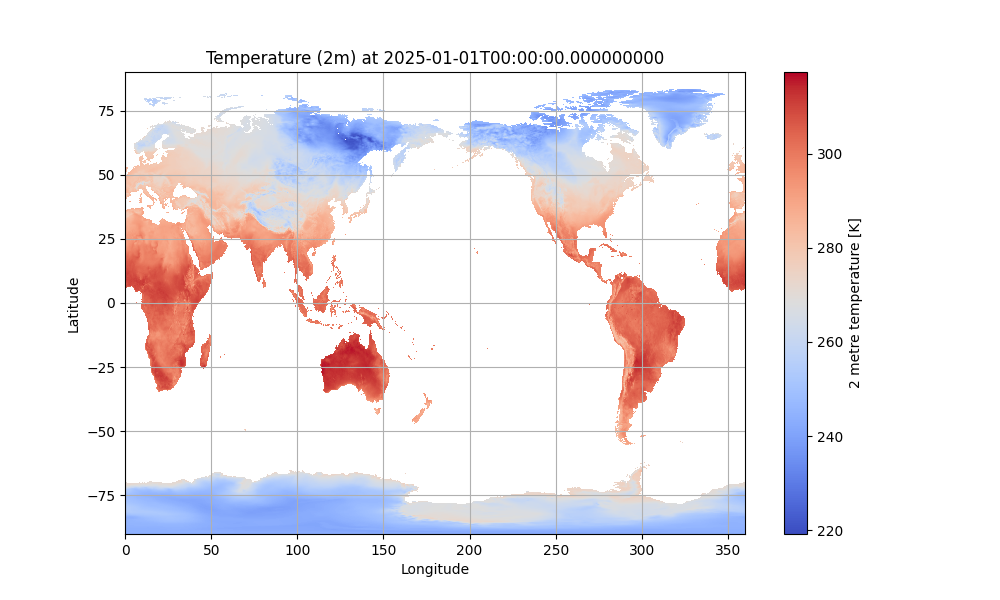
\includegraphics[width=0.85\textwidth]{images/era_t2m_2025_01_01_00.png}
    \caption{ERA5 2m air temperature on January 1, 2025 at 00 UTC. The temperature field is visualized from the high-resolution Zarr archive.}
    \label{fig:era_t2m_2025_01_01_00}
\end{figure}

%------------------------------------------------------------------------------
%
%------------------------------------------------------------------------------
\subsection{ZARR Structure and Conversion with Xarray}

The practical use of Zarr is illustrated clearly in the provided notebook, which details the process of converting NetCDF files, commonly used for meteorological data such as ERA5 temperature data (T2M), into a Zarr format compatible with Anemoi.

Initially, we load a NetCDF dataset using Xarray, a Python library for handling multi-dimensional arrays effectively:

\begin{codeonly}{Open\_Era\_after\_Download}
import xarray as xr

# Load Dataset
ds = xr.open_dataset('era_t2m.nc')
print(ds)
\end{codeonly}

This step provides an overview of dataset variables and coordinates. For instance, to visualize temperature at the first time step:

\begin{codeonly}{Display\_ERA\_T2M\_Field}
import matplotlib.pyplot as plt

# Select First Time Step and Plot
t2m = ds['t2m'].isel(valid_time=0)
t2m.plot(cmap='coolwarm')
plt.title('ERA5 2m Temperatur (erste Zeitstufe)')
plt.show()
\end{codeonly}

The conversion from NetCDF to Zarr involves renaming the primary data variable (`t2m`) to `data` for compatibility with Anemoi, a data analysis and visualization framework:

\begin{codeonly}{Convert\_to\_Zarr}
import os
from anemoi.datasets.data import open_dataset, add_dataset_path

# Rename Variable and Convert to Zarr
netcdf_file_path = "era_t2m.nc"
zarr_archive_path = "era_t2m.zarr"

ds_netcdf = xr.open_dataset(netcdf_file_path)
ds_renamed = ds_netcdf.rename_vars({'t2m': 'data'})
ds_renamed.to_zarr(zarr_archive_path, mode='w', compute=True, consolidated=True)
\end{codeonly}

After conversion, we inspect the resulting Zarr archive's contents:

\begin{codeonly}{Inspect\_ZARR\_File}
# Inspect Zarr Structure
ds_zarr = xr.open_zarr("era_t2m.zarr", consolidated=True)
print(ds_zarr)

# List Variables and Coordinates
print("Variables in Zarr Dataset:")
for var in ds_zarr.data_vars:
    print(f" - {var}")

print("\nCoordinates:")
for coord in ds_zarr.coords:
    print(f" - {coord}: shape={ds_zarr[coord].shape}")
\end{codeonly}

%------------------------------------------------------------------------------
%
%------------------------------------------------------------------------------
\begin{figure}[ht]
    \centering
    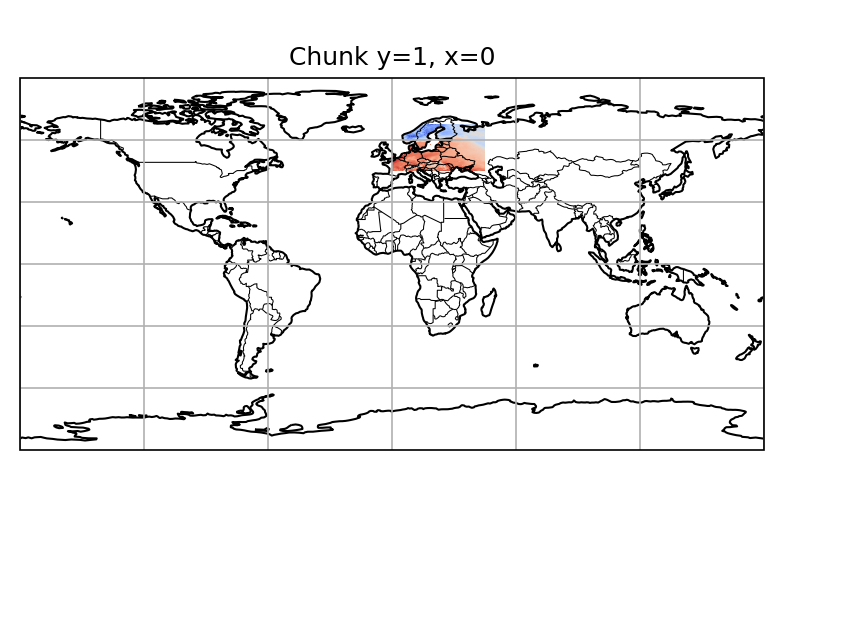
\includegraphics[width=0.85\textwidth]{images/era_zarr_1_0.png}
    \caption{ERA5 2m Temperature from Zarr Chunk at Index \texttt{(y=1, x=0)}.
    The chunk covers Central Europe and is extracted from the Zarr archive.
    Visualization uses \texttt{Cartopy} with coastlines and borders for orientation.}
    \label{fig:era-zarr-chunk-1-0}
\end{figure}

%------------------------------------------------------------------------------
%
%------------------------------------------------------------------------------
Visualization of data stored within the Zarr archive is straightforward, leveraging Xarray's built-in plotting capabilities:

\begin{codeonly}{Visualize\_Zarr}
# Visualize Zarr Data
import matplotlib.pyplot as plt

# Select First Time Step for Visualization
time_slice = ds_zarr.isel(valid_time=0)
time_slice.data.plot(cmap='coolwarm')
plt.title(f"Temperature (2m) at {str(time_slice.valid_time.values)}")
plt.xlabel("Longitude")
plt.ylabel("Latitude")
plt.grid(True)
plt.show()
\end{codeonly}

Thus, Zarr provides an optimized storage solution facilitating efficient data handling, which integrates seamlessly with Anemoi for high-performance analysis and visualization.

Lets have a quick look at the structure of the ZARR directory. 

\begin{lstlisting}
(ropy_wsl) rolan@White-WIN:~/all/python_and_ml_tutorial/code/code16/era_t2m.zarr\$ ll
total 0
drwxrwxrwx 1 rolan rolan 512 May 24 10:27 data
drwxrwxrwx 1 rolan rolan 512 May 24 10:27 latitude
drwxrwxrwx 1 rolan rolan 512 May 24 10:27 longitude
drwxrwxrwx 1 rolan rolan 512 May 24 10:27 number
drwxrwxrwx 1 rolan rolan 512 May 24 10:27 valid_time
\end{lstlisting}

and in the data/ directory we find: 
\begin{lstlisting}
(ropy_wsl) rolan@White-WIN:~/all/python_and_ml_tutorial/code/code16/era_t2m.zarr\$ cd data
(ropy_wsl) rolan@White-WIN:~/all/python_and_ml_tutorial/code/code16/era_t2m.zarr/data\$ ls
0.0.0  0.5.0  1.2.0  1.7.0  2.4.0  3.1.0  3.6.0  4.3.0  5.0.0  5.5.0  6.2.0  6.7.0  7.4.0
0.0.1  0.5.1  1.2.1  1.7.1  2.4.1  3.1.1  3.6.1  4.3.1  5.0.1  5.5.1  6.2.1  6.7.1  7.4.1
0.0.2  0.5.2  1.2.2  1.7.2  2.4.2  3.1.2  3.6.2  4.3.2  5.0.2  5.5.2  6.2.2  6.7.2  7.4.2
0.0.3  0.5.3  1.2.3  1.7.3  2.4.3  3.1.3  3.6.3  4.3.3  5.0.3  5.5.3  6.2.3  6.7.3  7.4.3
0.0.4  0.5.4  1.2.4  1.7.4  2.4.4  3.1.4  3.6.4  4.3.4  5.0.4  5.5.4  6.2.4  6.7.4  7.4.4
...
\end{lstlisting}

{\bf Chunk Content Example.} To better understand how Zarr stores data internally, we examined a single chunk file named \texttt{0.0.0} within the directory \texttt{era\_t2m.zarr/data/}. This chunk stores a sub-array of shape $(4,\ 226,\ 450)$, corresponding to the first four time steps and the northwestern corner of the global grid.

Most values in the upper part of the chunk are \texttt{NaN} due to the presence of land–sea masks or undefined polar values, but valid temperature values in Kelvin appear in the lower latitudes of this block:

\begin{verbatim}
Chunk shape: (4, 226, 450)
Sample values (in Kelvin):
[[[     nan  ...  271.6  271.5]
  ...
  [     nan  ...  271.7  271.6]]
 ...
 [[     nan  ...  267.5  267.4]]]
\end{verbatim}


%==============================================================================
%
%==============================================================================
\section{Building an Icosahedral Graph with Anemoi}

Very similarly to the ICON model framework, Anemoi provides tools to generate geodesic or icosahedral graphs suited for global data analysis. These graphs are constructed from refined icosahedrons, making them highly suitable for earth system modeling, weather prediction, and geospatial machine learning.

%------------------------------------------------------------------------------
%
%------------------------------------------------------------------------------
\subsection{Generating the Graph Structure}

{\bf GraphCreator, TriNodes, KNNEdges, and OmegaConf.}
The graph generation is controlled via a configuration dictionary, passed to the \texttt{GraphCreator} class. It defines the node layout and edge construction logic:

\begin{codeonly}{Graph Creation with GraphCreator, TriNodes, and KNNEdges}
from anemoi.graphs.create import GraphCreator
from omegaconf import OmegaConf

config = OmegaConf.create({
    "nodes": {
        "ico_nodes": {
            "node_builder": {
                "_target_": "anemoi.graphs.nodes.builders.from_refined_icosahedron.TriNodes",
                "resolution": 4,
                "name": "ico_nodes"
            },
            "attributes": {}
        }
    },
    "edges": [
        {
            "source_name": "ico_nodes",
            "target_name": "ico_nodes",
            "edge_builders": [
                {
                    "_target_": "anemoi.graphs.edges.builder.KNNEdges",
                    "num_nearest_neighbours": 6
                }
            ]
        }
    ]
})

creator = GraphCreator(config)
graph = creator.create()
\end{codeonly}

%------------------------------------------------------------------------------
%
%------------------------------------------------------------------------------
{\bf TriNodes and resolution.}
The \texttt{TriNodes} builder constructs a set of points on the surface of the globe by refining an icosahedron. The \texttt{resolution} parameter controls the granularity: higher values lead to finer meshes.

{\bf KNNEdges and edge\_index.}
The \texttt{KNNEdges} builder establishes connections between each node and its nearest neighbors. The resulting edge list is stored as \texttt{edge\_index} in the graph structure.

%------------------------------------------------------------------------------
%
%------------------------------------------------------------------------------
\subsection{Visualization on a 2D Map}

The graph can be rendered on a 2D world map using Cartopy. Each node is plotted based on its latitude and longitude, and edges are drawn as lines connecting the connected nodes.

\begin{figure}[htbp]
    \centering
    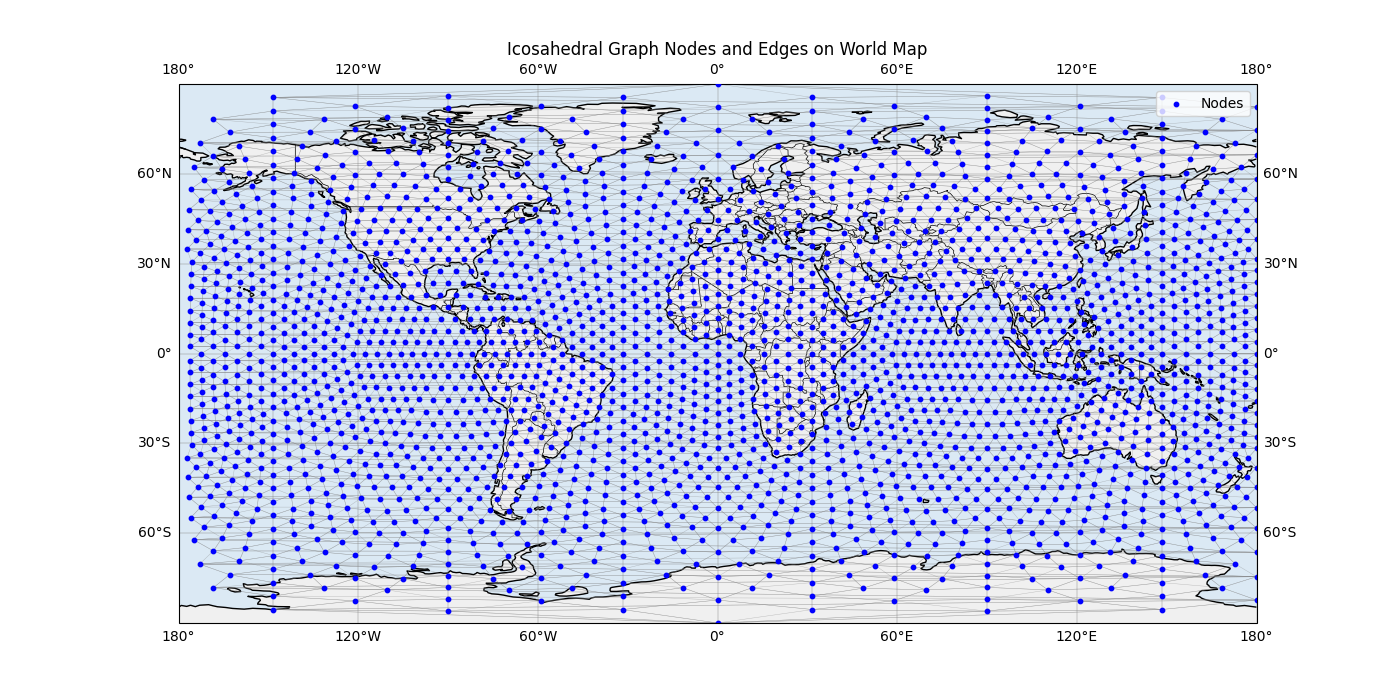
\includegraphics[width=0.92\textwidth]{images/anemoi_graph_1.png}
    \caption{Icosahedral graph constructed using TriNodes with resolution 4. The nodes and their nearest-neighbor edges are plotted on a global Plate Carree map.}
    \label{fig:anemoi-graph-platecarree}
\end{figure}

%------------------------------------------------------------------------------
%
%------------------------------------------------------------------------------
\subsection{Orthographic Globe Projection}

{\bf Orthographic and Geodetic.}
To emphasize the spherical nature of the graph, a globe visualization is generated using the orthographic projection. This highlights how the graph tiles the earth's surface in a nearly uniform manner.

\begin{figure}[htbp]
    \centering
    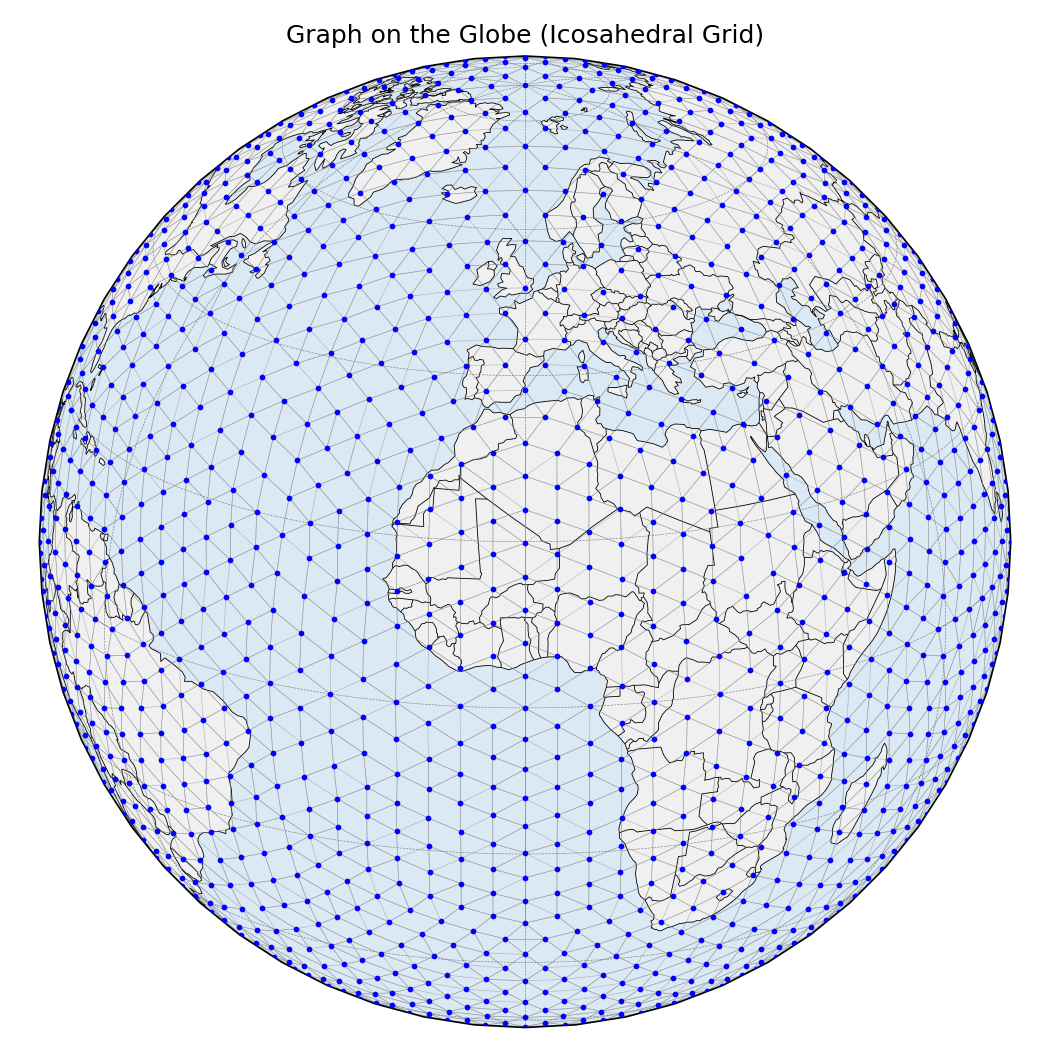
\includegraphics[width=0.6\textwidth]{images/anemoi_graph_2.png}
    \caption{The same Anemoi icosahedral graph visualized on a globe using orthographic projection and geodetic edge rendering.}
    \label{fig:anemoi-graph-globe}
\end{figure}

{\bf Great Circle and edge curvature.}
Edges on the globe are rendered using great-circle arcs to reflect the shortest path between nodes on a sphere, implemented by setting the transform to \texttt{ccrs.Geodetic()}. This workflow shows how Anemoi enables modular, reproducible graph construction with spherical geometry, suitable for earth system data and machine learning models.


%==============================================================================
%
%==============================================================================
\section{Hands-On Datasets, Validation, Training With Anemoi}

We have already shown that creating zarr is possible by several tools. Anemoi uses these tools, but has created its own interface to add all the metadata in a format which is then used by its training modules. 

\begin{codeonly}{Create ZARR from GRIB}
(ropy_wsl) rolan@White-WIN:~/all/python_and_ml_tutorial/code/code16\$ anemoi-datasets create download.yaml download.zarr --overwrite
2025-05-24 14:49:15 INFO Task init((),{}) starting
2025-05-24 14:49:16 INFO Setting flatten_grid=True in config
2025-05-24 14:49:16 INFO Setting ensemble_dimension=2 in config
2025-05-24 14:49:16 INFO Setting flatten_grid=True in config
2025-05-24 14:49:16 INFO Setting ensemble_dimension=2 in config
2025-05-24 14:49:17 INFO {'start': datetime.datetime(2024, 3, 1, 13, 0), 'end': datetime.datetime(2024, 3, 2, 12, 0), 'frequency': '24h', 'group_by': 'monthly'}
2025-05-24 14:49:17 INFO Groups(dates=1,StartEndDates(2024-03-01 13:00:00..2024-03-02 12:00:00 every 1 day, 0:00:00))
2025-05-24 14:49:17 INFO Groups: Groups(dates=1,StartEndDates(2024-03-01 13:00:00..2024-03-02 12:00:00 every 1 day, 0:00:00))
2025-05-24 14:49:25 INFO Minimal input for 'init' step (using only the first date) : GroupOfDates(dates=['2024-03-01T13:00:00'])
2025-05-24 14:49:25 INFO JoinResult: 1 dates (2024-03-01T13:00)
  grib(GroupOfDates(dates=['2024-03-01T13:00:00']))
2025-05-24 14:49:25 INFO Config loaded ok:
2025-05-24 14:49:25 INFO Found 1 datetimes.
2025-05-24 14:49:25 INFO Dates: Found 1 datetimes, in 1 groups:
2025-05-24 14:49:25 INFO Missing dates: 0
2025-05-24 14:49:27 INFO Found 1 variables : z_1000.
2025-05-24 14:49:27 INFO Found 1 ensembles : 0.
2025-05-24 14:49:27 INFO gridpoints size: [1038240, 1038240]
2025-05-24 14:49:27 INFO resolution=0.25
2025-05-24 14:49:27 INFO total_shape = [1, 1, 1, 1038240]
2025-05-24 14:49:27 INFO chunks=(1, 1, 1, 1038240)
2025-05-24 14:49:27 INFO Creating Dataset 'download.zarr', with total_shape=[1, 1, 1, 1038240], chunks=(1, 1, 1, 1038240) and dtype='float32'
2025-05-24 14:49:27 WARNING Dataset name error: the dataset name 'download' does not follow naming convention. Does not match ^(\w+)-([\w-]+)-(\w+)-(\w+)-(\d\d\d\d)-(\d\d\d\d)-(\d+h|\d+m)-v(\d+)-?([a-zA-Z0-9-]+)?\$
2025-05-24 14:49:27 INFO Number of years 0 < 10, leaving out 20%. end=numpy.datetime64('2024-03-01T13:00:00')
2025-05-24 14:49:28 INFO Will compute statistics from 2024-03-01T13:00:00 to 2024-03-01T13:00:00
2025-05-24 14:49:28 INFO Task init((),{}) completed (0:00:12.152389)
2025-05-24 14:49:28 INFO Task load((),{}) starting
2025-05-24 14:49:28 INFO {'end': '2024-03-02T12:00:00', 'frequency': '24h', 'group_by': 'monthly', 'start': '2024-03-01T13:00:00'}
2025-05-24 14:49:28 INFO Groups(dates=1,StartEndDates(2024-03-01 13:00:00..2024-03-02 12:00:00 every 1 day, 0:00:00))
2025-05-24 14:49:28 INFO Loading array shape=(1, 1, 1, 1038240), indexes=1
Loading 0/1: 100 1/1 [00:00<00:00, 279.19it/s]
2025-05-24 14:49:28 INFO Computing statistics for (1, 1, 1, 1038240) array
2025-05-24 14:49:28 INFO Statistics computed for 1 variables.
2025-05-24 14:49:28 INFO Flush data array
2025-05-24 14:49:28 INFO Flushed data array
2025-05-24 14:50:17 INFO Saving file at /6_Anemoi_Training.ipynb
2025-05-24 14:50:29 INFO Name               : /data
Type               : zarr.core.Array
Data type          : float32
Shape              : (1, 1, 1, 1038240)
Chunk shape        : (1, 1, 1, 1038240)
Order              : C
Read-only          : True
Compressor         : Blosc(cname='lz4', clevel=5, shuffle=SHUFFLE, blocksize=0)
Store type         : zarr.storage.DirectoryStore
No. bytes          : 4152960 (4.0M)
No. bytes stored   : 1968080 (1.9M)
Storage ratio      : 2.1
Chunks initialized : 1/1

2025-05-24 14:50:29 INFO Task load((),{}) completed (0:01:01.203754)
2025-05-24 14:50:29 INFO Task finalise((),{}) starting
2025-05-24 14:50:29 INFO Variables minimum maximum mean stdev has_nans
z_1000 -4286.61 3106.39 715.22 1190.58 0.00
2025-05-24 14:50:29 INFO Wrote statistics in download.zarr
Computing size of download.zarr: 16it [00:00, 128.73it/s]
2025-05-24 14:50:29 INFO Total size: 2 MiB
2025-05-24 14:50:29 INFO Total number of files: 75
2025-05-24 14:50:29 INFO Task finalise((),{}) completed (0:00:00.657181)
2025-05-24 14:50:29 INFO Task init_additions((),{}) starting
2025-05-24 14:50:29 WARNING No delta found in kwargs, no additions will be computed.
2025-05-24 14:50:29 INFO Task init_additions((),{}) completed (0:00:00.000138)
2025-05-24 14:50:29 INFO Task run_additions((),{}) starting
2025-05-24 14:50:29 WARNING No delta found in kwargs, no additions will be computed.
2025-05-24 14:50:29 INFO Task run_additions((),{}) completed (0:00:00.000105)
2025-05-24 14:50:29 INFO Task finalise_additions((),{}) starting
2025-05-24 14:50:29 WARNING No delta found in kwargs, no additions will be computed.
Computing size of download.zarr: 16it [00:00, 130.81it/s]
2025-05-24 14:50:30 INFO Total size: 2 MiB
2025-05-24 14:50:30 INFO Total number of files: 75
2025-05-24 14:50:30 INFO Task finalise_additions((),{}) completed (0:00:00.226333)
2025-05-24 14:50:30 INFO Task patch((),{}) starting
2025-05-24 14:50:30 INFO Remove _create_yaml_config
2025-05-24 14:50:30 INFO Dataset changed by patch
2025-05-24 14:50:30 INFO Task patch((),{}) completed (0:00:00.364498)
2025-05-24 14:50:30 INFO Task cleanup((),{}) starting
2025-05-24 14:50:30 INFO Task cleanup((),{}) completed (0:00:00.007262)
2025-05-24 14:50:30 INFO Task verify((),{}) starting
2025-05-24 14:50:30 INFO Verifying dataset at download.zarr
2025-05-24 14:50:30 INFO download.zarr
2025-05-24 14:50:30 INFO Task verify((),{}) completed (0:00:00.021160)
2025-05-24 14:50:30 INFO Create completed in 1 minute 14 seconds
(ropy_wsl) rolan@White-WIN:~/all/python_and_ml_tutorial/code/code16\$
\end{lstlisting}

You can then inspect the dataset you generated: 
\begin{codeonly}{Inspect generated ZARR}
(ropy_wsl) rolan@White-WIN:~/all/python_and_ml_tutorial/code/code16\$ anemoi-datasets inspect download.zarr
Path          : download.zarr
Format version: 0.30.0

Start      : 2024-03-01 13:00
End        : 2024-03-01 13:00
Frequency  : 1d
Missing    : 0
Resolution : 0.25
Field shape: [721, 1440]

$1 \times 1 \times 1 \times 1,038,240$
Size       : 2 MiB (2 MiB)
Files      : 75
\begin{tabular}{|c|c|r|r|r|r|}
\hline
\textbf{Index} & \textbf{Variable} & \textbf{Min} & \textbf{Max} & \textbf{Mean} & \textbf{Stdev} \\
\hline
0 & z\_1000 & -4286.61 & 3106.39 & 715.219 & 1190.58 \\
\hline
\end{tabular}
Dataset ready, last update 2 hours ago.
Statistics ready.
\end{codeonly}

We can validate a debug.yaml as follows: 

\begin{codeonly}{Validate YAML}
(ropy_wsl) rolan@White-WIN:~/all/python_and_ml_tutorial/code/code16\$ anemoi-training config validate --config-name debug.yaml
2025-05-24 17:00:42 INFO Validating configs.
2025-05-24 17:00:42 WARNING Note that this command is not taking into account if your config has set                     the config_validation flag to false.So this command will validate the config regardless of the flag.
2025-05-24 17:00:42 INFO Prepending current user directory (/mnt/c/Users/rolan/all/python_and_ml_tutorial/code/code16) to the search path.
2025-05-24 17:00:42 INFO Search path is now: [provider=anemoi-cwd-searchpath-plugin, path=/mnt/c/Users/rolan/all/python_and_ml_tutorial/code/code16, provider=hydra, path=pkg://hydra.conf, provider=main, path=/mnt/c/Users/rolan/all/ropy_wsl/lib/python3.12/site-packages/anemoi/training/commands]
2025-05-24 17:00:43 INFO Config files validated.
\end{codeonly}

And then training can be initiazized by: 

\begin{codeonly}{Training Initialization}
anemoi-training train --config-name=debug
\end{codeonly}




%==============================================================================
%
%==============================================================================
\section{Training Pipeline in Anemoi}

The training process in Anemoi is managed by the script \texttt{train.py} in the \texttt{anemoi-training} package. It implements a highly modular, Hydra-driven architecture built on top of PyTorch Lightning. The main orchestration is encapsulated in the \texttt{AnemoiTrainer} class, which configures, initializes, and runs model training and evaluation.

To get started, you can generate a default configuration file as we showed above. 

%------------------------------------------------------------------------------
%
%------------------------------------------------------------------------------
\subsection{Hydra Entry Point and Configuration}

The training is launched via a Hydra-decorated \texttt{main} function at the end of \texttt{train.py}. This function serves as the command-line entry point for Anemoi training jobs. Hydra parses the YAML configuration files into a nested \texttt{DictConfig} object and injects it into the trainer.

The \texttt{main} function's definition and entry point can be found here:
\url{https://github.com/ecmwf/anemoi-core/blob/main/training/src/anemoi/training/train/train.py#L497-L500}

\begin{codeonly}{Hydra Entry Point}
@hydra.main(version_base=None, config_path="../config", config_name="config")
def main(config: DictConfig) -> None:
AnemoiTrainer(config).train()
\end{codeonly}

The configuration system supports:
\begin{itemize}
\item Model and data module selection
\item Training hyperparameters
\item Graph and truncation settings
\item Logging, callbacks, and checkpointing
\end{itemize}

%------------------------------------------------------------------------------
%
%------------------------------------------------------------------------------
\subsection{AnemoiTrainer Class Overview}

The \texttt{AnemoiTrainer} class is the core wrapper for the entire experiment lifecycle. It performs validation and conversion of the Hydra configuration schema, sets up metadata, seeds, run IDs, and logging paths, constructs or loads graph and truncation data, initializes the data module and model via Hydra, and creates callbacks and loggers (MLflow, TensorBoard, W\&B).

The \texttt{AnemoiTrainer} class definition begins at:
\url{https://github.com/ecmwf/anemoi-core/blob/main/training/src/anemoi/training/train/train.py#L51-L494}

Many of these components are defined as \texttt{@cached\_property}, ensuring lazy and consistent instantiation. For instance, the properties for the datamodule, graph data, and model are defined as:

\begin{codeonly}{Core Cached Properties}
@property
def datamodule(self) -> Any: ... # Definition at https://github.com/ecmwf/anemoi-core/blob/main/training/src/anemoi/training/train/train.py#L101-L105
@property
def graph_data(self) -> HeteroData: ... # Definition at https://github.com/ecmwf/anemoi-core/blob/main/training/src/anemoi/training/train/train.py#L157-L162
@property
def model(self) -> pl.LightningModule: ... # Definition at https://github.com/ecmwf/anemoi-core/blob/main/training/src/anemoi/training/train/train.py#L190-L200
\end{codeonly}

%------------------------------------------------------------------------------
%
%------------------------------------------------------------------------------
\subsection{Model and Data Instantiation}

The model and data modules are instantiated dynamically from the YAML config using Hydra utilities within the \texttt{AnemoiTrainer} class. This allows complete flexibility, enabling different models and datasets to be specified per experiment without requiring code changes.

The instantiation of the model typically occurs in the \texttt{model} cached property:
\url{https://github.com/ecmwf/anemoi-core/blob/main/training/src/anemoi/training/train/train.py#L195-L199}

The instantiation of the datamodule occurs in the \texttt{datamodule} cached property:
\url{https://github.com/ecmwf/anemoi-core/blob/main/training/src/anemoi/training/train/train.py#L102-L104}

\begin{codeonly}{Dynamic Instantiation}
model_task = get_class(self.config.training.model_task) # See line 196
model = model_task(
   config=self.config,
   data_indices=self.data_indices,
   graph_data=self.graph_data,
   # ... other arguments ...
) # See lines 197-199

datamodule = instantiate( # See line 102
   convert_to_omegaconf(self.config).datamodule,
   convert_to_omegaconf(self.config),
   self.graph_data,
) # See lines 103-104
\end{codeonly}

%------------------------------------------------------------------------------
%
%------------------------------------------------------------------------------
\subsection{Training Execution via Lightning}

The actual training is launched by calling the \texttt{train()} method of the \texttt{AnemoiTrainer} class. This method constructs a \texttt{pl.Trainer} instance and calls its \texttt{fit()} method, leveraging PyTorch Lightning for the training loop management.

The \texttt{train} method is defined at:
\url{https://github.com/ecmwf/anemoi-core/blob/main/training/src/anemoi/training/train/train.py#L455-L494}

The \texttt{pl.Trainer} instance is initialized at:
\url{https://github.com/ecmwf/anemoi-core/blob/main/training/src/anemoi/training/train/train.py#L486-L493}

And the trainer.fit call that starts the training process is at:
\url{https://github.com/ecmwf/anemoi-core/blob/main/training/src/anemoi/training/train/train.py#L486}

\begin{codeonly}{Lightning Training Loop}
trainer = pl.Trainer( # Initialized at lines 489-493
	accelerator=self.accelerator,
	callbacks=self.callbacks,
	strategy=self.strategy,
	logger=self.loggers,
	max_epochs=self.config.training.max_epochs,
	# ... other arguments ...
)
trainer.fit( # Called at lines 495-498
	self.model,
	datamodule=self.datamodule,
	ckpt_path=None if self.load_weights_only else self.last_checkpoint,
)
\end{codeonly}

PyTorch Lightning handles the boilerplate of device placement, training/validation looping, and checkpointing. Logging is automatically integrated with MLflow or Weights \& Biases depending on the configuration.

%------------------------------------------------------------------------------
%
%------------------------------------------------------------------------------
\subsection{Configuration and Schema Management}

Anemoi uses configuration schemas defined in \texttt{schemas/base\_schema.py} to validate and standardize the structure of the configuration. This ensures consistency across model runs and supports reproducibility by recording full config metadata.

The main configuration schema definitions can be found here:
\url{https://github.com/ecmwf/anemoi-core/blob/main/training/src/anemoi/training/schemas/base_schema.py#L45}

Key components of the schema system include:
\begin{itemize}
\item \texttt{BaseSchema}: The primary validated configuration interface.
\item \texttt{UnvalidatedBaseSchema}: Used for more lenient configuration parsing, often during initial setup or debugging.
\item Conversion utilities: Ensure compatibility with OmegaConf and Hydra's internal data structures.
\end{itemize}

%------------------------------------------------------------------------------
%
%------------------------------------------------------------------------------
\subsection{Summary}

The Anemoi training pipeline brings together Hydra for flexible configuration, PyTorch Lightning for robust training infrastructure, and specific data tools for handling graph and weather model inputs. The \texttt{AnemoiTrainer} class encapsulates the orchestration of these components, making experiments declarative, reproducible, and modular.




